\chapter{Anexos}
\addcontentsline{toc}{chapter}

% ---- 1
\subsection*{Anexo 1: Carta de presentación}
\addcontentsline{toc}{subsection}{Anexo 1: Carta de presentación}
\label{anexo:carta_presentacion}
\parbox{\linewidth}{%
Documento adjunto con la carta de presentación formal del proyecto "Sistema de Gestión Integral Universitario".
(\href{https://drive.google.com/file/d/1ZiMqNbFV13NKYQdoq0BSWwP7N5zLHqEC/view?usp=sharing}{Abrir anexo})
}

% ---- 2
\subsection*{Anexo 2: Carta de intenciones}
\addcontentsline{toc}{subsection}{Anexo 2: Carta de intenciones}
\label{anexo:carta_intenciones}
\parbox{\linewidth}{%
Documento adjunto con la carta formal que expresa la intención de las partes involucradas.
(\href{https://docs.google.com/document/d/1mUg4rNGD-5bXCqqc1IveIhCw3kNjwFzT/edit?usp=sharing&ouid=101041738052125290143&rtpof=true&sd=true}{Abrir anexo})
}

% ---- 3
\subsection*{Anexo 3: Código de Ética}
\addcontentsline{toc}{subsection}{Anexo 3: Código de Ética}
\label{anexo:codigo_etica}
\parbox{\linewidth}{%
Código de ética a seguir por todos los miembros del proyecto.
(\href{https://drive.google.com/file/d/1UWY2H4dAQ1W3nxtcGwQE1XzGkuUX-IoS/view?usp=sharing}{Abrir anexo})
}

% ---- 4
\subsection*{Anexo 4: Propuesta del proyecto}
\addcontentsline{toc}{subsection}{Anexo 4: Propuesta del proyecto}
\label{anexo:propuesta_proyecto}
\parbox{\linewidth}{%
Propuesta formal del proyecto (empresa patrocinadora y alcances).
(\href{https://docs.google.com/document/d/13UJsHS4BudBLwkDqmcAJCtjnNyk6dAAS/edit?usp=sharing&ouid=101041738052125290143&rtpof=true&sd=true}{Abrir anexo})
}

% ---- 5
\subsection*{Anexo 5: Registro de actores del proyecto}
\addcontentsline{toc}{subsection}{Anexo 5: Registro de actores del proyecto}
\label{anexo:registro_actores}
\parbox{\linewidth}{%
Listado y roles de todos los actores del proyecto.
(\href{https://drive.google.com/file/d/1S9Q-E96NIDpG0EMDX2YKTTqEs6Od8mdS/view?usp=sharing}{Abrir anexo})
}

% ---- 6
\subsection*{Anexo 6: Formato de minutas de reunión}
\addcontentsline{toc}{subsection}{Anexo 6: Formato de minutas de reunión}
\label{anexo:formato_minutas}
\parbox{\linewidth}{%
Plantilla estándar para actas y acuerdos.
(\href{https://drive.google.com/drive/folders/1BHOoTcfT2bxG1wUy7kJ4X7yb6q9h27er?usp=sharing}{Abrir anexo})
}

% ---- 7
\subsection*{Anexo 7: WBS (Estructura de Desglose de Trabajo)}
\addcontentsline{toc}{subsection}{Anexo 7: WBS (Estructura de Desglose de Trabajo)}
\label{anexo:wbs}
\parbox{\linewidth}{%
Diagrama con la estructura jerárquica de entregables.
(\href{https://drive.google.com/drive/folders/1ttuiMCmFBvJN9ji7XTXY-opBWwPszsYA?usp=sharing}{Abrir anexo})
}

% ---- 8
\subsection*{Anexo 8: SRS}
\addcontentsline{toc}{subsection}{Anexo 8: SRS}
\label{anexo:documento_srs}
\parbox{\linewidth}{%
Especificación de Requerimientos de Software (funcionales y no funcionales).
(\href{https://drive.google.com/file/d/1oJmhAV7PfzoFyCYmLh3L8nMICLeYXLhq/view?usp=sharing}{Abrir anexo})
}

% ---- 9
\subsection*{Anexo 9: Modelo No Relacional}
\addcontentsline{toc}{subsection}{Anexo 9: Modelo No Relacional}
\label{anexo:modelo_no_relacional}
\parbox{\linewidth}{%
Modelo no relacional (Prisma).
(\href{https://drive.google.com/file/d/1ib_2B1VA6txi9h-J2I136l8i4TbnE690/view?usp=sharing}{Abrir anexo})
}

% ---- 10
\subsection*{Anexo 10: Diccionario de Datos (general)}
\addcontentsline{toc}{subsection}{Anexo 10: Diccionario de Datos (general)}
\label{anexo:diccionario_general}
\parbox{\linewidth}{%
Tablas, campos, tipos, restricciones y relaciones del sistema.
(\href{https://drive.google.com/file/d/1sHDwVC5bjJg16aMmE7ue0gawE14cJS49/view?usp=sharing}{Abrir anexo})
}

% ---- 11
\subsection*{Anexo 11: Formulario de gestión de cambios}
\addcontentsline{toc}{subsection}{Anexo 11: Formulario de gestión de cambios}
\label{anexo:formulario_gestion_de_cambios}
\parbox{\linewidth}{%
Formulario para solicitar/analizar/aprobar cambios (alcance, cronograma, recursos).
(\href{https://drive.google.com/file/d/1LlylabUQ4ncxDJ_cMAvHNNz0IbQ720eB/view?usp=sharing}{Abrir anexo})
}

% ---- 12
\subsection*{Anexo 12: Carpeta de firmas}
\addcontentsline{toc}{subsection}{Anexo 12: Carpeta de firmas}
\label{anexo:carpeta_firmas}
\parbox{\linewidth}{%
Documentos originales firmados (aprobaciones, minutas, acuerdos).
(\href{https://drive.google.com/drive/folders/1RyhaHzP8_-uZjUJkA3g5nfkAvk997w2Y?usp=sharing}{Abrir anexo})
}

% ---- 13
\subsection*{Anexo 13: Desarrollo}
\addcontentsline{toc}{subsection}{Anexo 13: Desarrollo}
\label{anexo:desarrollo}
\parbox{\linewidth}{%
Evidencias de vistas y prototipos funcionales.
(\href{https://drive.google.com/drive/folders/1Gh8xDngg0TndL0D7ia3ZEBqxs9TuCOrf?usp=sharing}{Abrir anexo})
}

% ---- 14
\subsection*{Anexo 14: Diccionario de Datos — Evidencias SINAES}
\addcontentsline{toc}{subsection}{Anexo 14: Diccionario de Datos — Evidencias SINAES}
\label{anexo:dicc_evidencias}
\parbox{\linewidth}{%
Estructura y metadatos del módulo de evidencias SINAES.
(\href{https://drive.google.com/file/d/1aWdZiAq-vZ_1Ty9TgkDgT_mCuPRHtm_o/view?usp=drive_link}{Abrir anexo})
}

% ---- 15
\subsection*{Anexo 15: Diccionario de Datos — Tiempos de Jornada}
\addcontentsline{toc}{subsection}{Anexo 15: Diccionario de Datos — Tiempos de Jornada}
\label{anexo:dicc_jornada}
\parbox{\linewidth}{%
Estructura y reglas de cálculo del módulo de tiempos de jornada.
(\href{https://drive.google.com/file/d/1hmq_H_os67XBwliWEogt59qXKPFq964F/view?usp=drive_link}{Abrir anexo})
}

% ---- 16
\subsection*{Anexo 16: Glosario}
\addcontentsline{toc}{subsection}{Anexo 16: Glosario}
\label{anexo:glosario}
\parbox{\linewidth}{%
Glosario de términos y abreviaturas del proyecto.
(\href{https://drive.google.com/file/d/18UFM7d1duhJpcXTDCmMAK4PnTFuqFT9k/view?usp=sharing}{Abrir anexo})
}

% ---- 17
\subsection*{Anexo 17: Análisis}
\addcontentsline{toc}{subsection}{Anexo 17: Análisis}
\label{anexo:analisis}
\parbox{\linewidth}{%
Documentos de análisis, supuestos y límites.
(\href{https://drive.google.com/file/d/1S_cPKigSkLcA06b0DwnT0mBnKnIiOwZz/view?usp=sharing}{Abrir anexo})
}

% ---- 18
\subsection*{Anexo 18: Diseño}
\addcontentsline{toc}{subsection}{Anexo 18: Diseño (diagramas)}
\label{anexo:diseno}
\parbox{\linewidth}{%
Diagramas y artefactos de diseño (UI/arquitectura).
(\href{https://drive.google.com/file/d/1fP3GDwJTx6le_CSUnIHpsyVAWys5i6Xe/view?usp=sharing}{Abrir anexo})
}

\subsection*{Anexo 19: Diagrama Evidencias SINAES}
\label{anexo:anexo19}
Diagrama general del módulo de Evidencias.\\[2pt]
\textbf{Enlace:} \href{https://drive.google.com/file/d/1JOyRg4BCDVRNGavIcEJBhe_vZfon9DQJ/view?usp=sharing}{Abrir anexo}

\subsection*{Anexo 20: Diagrama Tiempos de Jornada}
\label{anexo:anexo20}
Diagrama general del módulo de Tiempos de Jornada.\\[2pt]
\textbf{Enlace:} \href{https://drive.google.com/file/d/1e3sLb27zRPAvATex8cs8AFXy211b11QI/view?usp=sharing}{Abrir anexo}

\subsection*{Anexo 21
: Cronograma de Sprints}

En la Figura \ref{fig:cronograma-sprints} se presenta el cronograma de sprints planificado para el proyecto de \textbf{Ingeniería en Sistemas II}, el cual contempla tanto los avances técnicos como la documentación asociada a los módulos de \textit{Evidencias SINAES} y \textit{Tiempos de Jornada}.  
Este cronograma sigue la estructura de entregables definidos en los sprints, permitiendo visualizar el estado (Completado, En Proceso, Pendiente) y las fechas clave de ejecución.

Versión digital:  
\href{https://drive.google.com/drive/folders/19OdLKElV0hTGwz3Frv35W6f6GwTeN_qK?usp=sharing} {Abrir cronograma}

\begin{figure}[H]
    \centering
    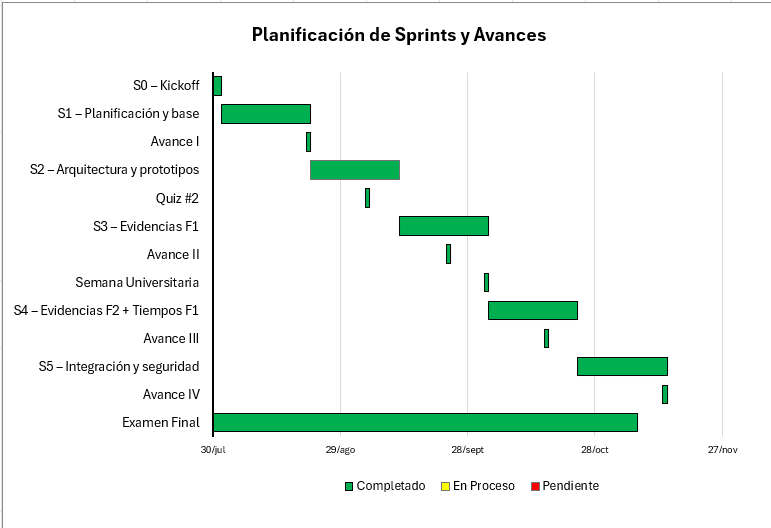
\includegraphics[width=\textwidth]{figs/cronograma (2).png}
    \caption{Cronograma de Sprints del Proyecto Ingeniería en Sistemas II.}
    \label{fig:cronograma-sprints}
\end{figure}
